\chapter{Testbenches} \label{ch:Testbenches}\index{testbench}
\chapterquote{Nothing inside me belongs to me, all is Yours. In returning that which belongs to You, what does it cost to me?}{Kabeer}

\graphicspath{{Chapters/Testbenches/Figures/}}
\lstinputpath{Codes-Verilog/Chapter-Testbenches/VerilogCodes} %path is defined in mypreamble

\section{Introduction}

In previous chapters, we generated the simulation waveforms using modelsim, by providing the input signal values manually; if the number of input signals are very large and/or we have to perform simulation several times, then this process can be quite complex, time consuming and irritating. Suppose input is of 10 bit, and we want to test all the possible values of input i.e. $2^{10}-1$, then it is impossible to do it manually. In such cases, testbenches are very useful; also, the tested designs are more reliable and prefer by the clients as well. Further, with the help of testbenches, we can generate results in the form of csv (comma separated file), which can be used by other softwares for further analysis e.g. Python, Excel and Matlab etc.  

\textbf{Since testbenches are used for simulation purpose only (not for synthesis), therefore full range of Verilog constructs can be used e.g. keywords `for', 'display' and `monitor' etc. can be used for writing testbenches.}

\textbf{Modelsim-project is created in this chapter for simulations}, which allows the relative path to the files with respect to project directory as shown in Section \ref{sec_read_data_from_file}. Simulation can be run without creating the project, but we need to provide the full path of the files as shown in Line 25  of Listing \ref{verilog:read_file_ex}. 

Lastly, mixed modeling is not supported by Altera-Modelsim-starter version, i.e. Verilog designs with VHDL and vice-versa can not be compiled in this version of Modelsim. For mixed modeling, we can use Active-HDL software as discussed in Chapter \ref{ch:OverView}.

\section{Testbench for combinational circuits}\index{testbench!combinational circuits}

In this section, various testbenches for combinational circuits are shown, whereas testbenches for sequential circuits are discussed in next section. For simplicity of the codes and better understanding, a simple half adder circuit is tested using various simulation methods. 

\subsection{Half adder}
Listing \ref{verilog:half_adder.v} shows the Verilog code for the half adder which is tested using different methods, 

\lstinputlisting[
language = Verilog,
caption    = {Half adder},
label      = {verilog:half_adder.v}
]{half_adder.v}
%
%
\subsection{Testbench with `initial block'}\index{initial}\index{testbench!initial}

Note that, testbenches are written in separate Verilog files as shown in Listing \ref{verilog:half_adder_tb.v}. Simplest way to write a testbench, is to invoke the `design for testing' in the testbench and provide all the input values inside the `initial block', as explained below, 

\begin{explanation}[Listing \ref{verilog:half_adder_tb.v}]
	In this listing, a testbench with name `half\_adder\_tb' is defined at Line 5. Note that, ports of the testbench is always empty i.e. no inputs or outputs are defined in the definition (see Line 5). Then 4 signals are defined i.e. a, b, sum and carry (Lines 7-8); these signals are then connected to actual half adder design using structural modeling (see Line 13). Lastly, different values are assigned to input signals e.g. `a' and `b' at lines 18 and 19 respectively. 
	
	\begin{noNumBox}
		`Initial block' is used at Line 15, which is executed only once, and terminated when the last line of the block executed i.e. Line 32. Hence, when we press run-all button in Fig. \ref{fig:half_adder_tb}, then simulation terminated after 60 ns (i.e. does not run forever). 
	\end{noNumBox}
	In Line 19, value of `b' is 0, then it changes to `1' at Line 23, after a delay of `period' defined at Line 20. The value of period is `20 (Line 11) * timescale (Line 3) = 20 ns'. In this listing all the combinations of inputs are defined manually i.e. 00, 01, 10 and 11; and the results are shown in Fig. \ref{fig:half_adder_tb}, also corresponding outputs i.e. sum and carry are shown in the figure. 
	
	\textbf{To generate the waveform, first compile the `half\_adder.v and then `half\_adder\_tb.v' (or compile both the file simultaneously.). Then simulate the half\_adder\_tb.v file. Finally, click on `run all' button (which will run the simulation to maximum time i.e. 80 ns)and then click then `zoom full' button (to fit the waveform on the screen), as shown in Fig. \ref{fig:half_adder_tb}.}
\end{explanation}

\lstinputlisting[
language = Verilog,
caption    = {Simple testbench for half adder},
label      = {verilog:half_adder_tb.v}
]{half_adder_tb.v}

\begin{figure}[!h]
	\centering
	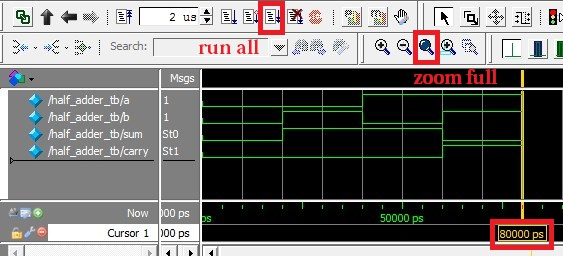
\includegraphics[scale=0.6]{half_adder_tb}
	\caption{Simulation results for Listing \ref{verilog:half_adder_tb.v}}
	\label{fig:half_adder_tb}
\end{figure}
%
%
\subsection{Testbench with `always' block} \label{sec:tb_with_process_statement}\index{always}\index{testbench!always}
In Listing \ref{verilog:half_adder_procedural_tb}, `always' statement is used in the testbench; which includes the input values along with the corresponding output values.  If the specified outputs are not matched with the output generated by half-adder, then errors will be displayed. \textbf{Note that in the testbenches, the `always' statement can be written with or without the sensitivity list as shown in Listing \ref{verilog:half_adder_procedural_tb}.}
\begin{noNumBox}
	Unlike `initial' block, the `always' block executes forever (if not terminated using `stop' keyword). The statements inside the `always' block execute sequentially; and after the execution of last statement, the execution begins again from the first statement of the `always' block. 
\end{noNumBox}
%
\begin{explanation}[Listing \ref{verilog:half_adder_procedural_tb}]
	The listing is same as previous Listing \ref{verilog:half_adder_tb.v}, but `always block' is used instead of `initial block', therefore we can provide the sensitive list to the design (Line 28) and gain more control over the testing. A continuous clock is generated in Lines 19-26 by not defining the sensitive list to always-block (Line 19). This clock is used by Line 28. Also, some messages are also displayed if the outcome of the design does not match with the desire outcomes (Lines 35-36). In this way, we can find errors just by reading the terminal (see Fig. \ref{fig:half_adder_process_error_tb}), instead of visualizing the whole waveform, which can be very difficult if the results are too long (see Fig. \ref{fig:half_adder_process_tb}). \textbf{Also, Lines 35-36 can be added in `initial-block' of Listing \ref{verilog:half_adder_tb.v} as well.}
\end{explanation}

\index{testbench!stop}\index{stop}
\lstinputlisting[
language = Verilog,
caption    = {Testbench with procedural statement},
label      = {verilog:half_adder_procedural_tb}
]{half_adder_procedural_tb.v}
%

\begin{figure}[!h]
	\centering
	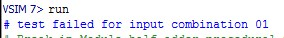
\includegraphics[scale=0.9]{half_adder_process_error_tb}
	\caption{Error generated by Listing \ref{verilog:half_adder_procedural_tb}}
	\label{fig:half_adder_process_error_tb}
\end{figure}

\begin{figure}[!h]
	\centering
	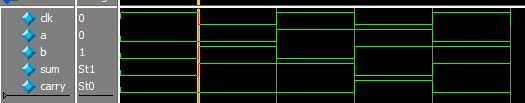
\includegraphics[scale=0.8]{half_adder_process_tb}
	\caption{Simulation results for Listing \ref{verilog:half_adder_procedural_tb}}
	\label{fig:half_adder_process_tb}
\end{figure}



\subsection{Read data from file} \label{sec_read_data_from_file}\index{testbench!read}
%
In this section, data is read from file `read\_file\_ex.txt' and displayed in simulation results. Date stored in the file is shown in Fig. \ref{fig:read_file_table_ex}. 

\begin{figure}[!h]
	\centering
	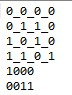
\includegraphics[scale=0.9]{read_file_table_ex}
	\caption{Data in file  `read\_file\_ex.txt'}
	\label{fig:read_file_table_ex}
\end{figure}

\begin{explanation}[Listing \ref{verilog:read_file_ex}]
	In the listing, `integer i (Line 16)' is used in the `for loop (Line 28)' to read all the lines of file `read\_file\_ex.txt'. Data can be saved in `binary' or `hexadecimal format'. Since data is saved in `binary format', therefor `readmemb' (Line 23) is used to read it. For `hexadecimal format', we need to use keyword `readmemh'. Read comments for further details of the listing. Data read by the listing is displayed in Fig. \ref{fig:read_file_ex}.  
\end{explanation}

\lstinputlisting[
language = Verilog,
caption    = {Read data from file},
label      = {verilog:read_file_ex}
]{read_file_ex.v}

\begin{figure}[!h]
	\centering
	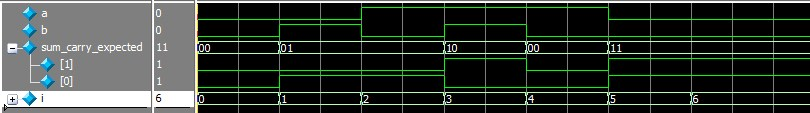
\includegraphics[width=\textwidth]{read_file_ex}
	\caption{Simulation results of Listing \ref{verilog:read_file_ex} }
	\label{fig:read_file_ex}
\end{figure}
%
%
\subsection{Write data to file}\index{testbench!write}

In this part, different types of values are defined in Listing \ref{verilog:write_file_ex.v} and then stored in the file. 

\begin{explanation}[Listing \ref{verilog:write_file_ex.v}]
	To write the data to the file, first we need to define an `integer' as shown in Line 14, which will work as buffer for open-file (see Line 28). Then data is written in the files using `fdisplay' command, and rest of the code is same as Listing  \ref{verilog:read_file_ex}.  
\end{explanation}
%
%
\lstinputlisting[
language = Verilog,
caption    = {Write data to file},
label      = {verilog:write_file_ex.v}
]{write_file_ex.v}

%
\begin{figure}[!h]
	\centering
	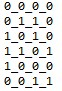
\includegraphics[scale=0.9]{write_file_table_ex}
	\caption{Data in file  `write\_file\_ex.txt'}
	\label{fig:write_file_table_ex}
\end{figure}

\section{Testbench for sequential designs}\index{testbench!sequential circuits}\index{testbench!save data to file}
In previous sections, we read the lines from one file and then saved those line in other file using `for loop'. Also, we saw use of `initial' and `always' blocks. In this section, we will combine all the techniques together to save the results of Mod-M counter, which is an example of `sequential design'. The Mod-m counter is discussed in Listing \ref{verilog:modMCounter}. Testbench for this listing is shown in Listing \ref{verilog:modMCounter_tb} and the waveforms are illustrated in Fig. \ref{fig:monitor_waveform}.

\begin{explanation}[Listing \ref{verilog:modMCounter_tb}]
	In the testbench following operations are performed, 
	\begin{enumerate}
		\item Simulation data is saved on the terminal and saved in a file. Note that, \textbf{`monitor/fmonitor'} keyword\index{testbench!monitor}\index{testbench!fmonitor}\index{monitor}\index{fmonitor} can be used in the \textbf{`initial' block}, which can track the changes in the signals as shown in Lines 98-108 and the output is shown in Fig. \ref{fig:monitor_error}. In the figure we can see that the `error' message is displayed two time (but the error is at one place only), as `monitor' command checks for the transition in the signal as well. 
		
		If we want to track only final results, then \textbf{`display/fdisplay'}\index{testbench!display}\index{testbench!fdisplay}\index{display}\index{fdisplay} command can be used inside the \textbf{always block} as shown in Lines 110-124 (Uncomment these lines and comment Lines 98-108). Output is show in Fig. \ref{fig:error_neg_edge_csv}. \textbf{Note that, it is very easy to look for errors in the terminal/csv file as compare to finding it in the waveforms.} 
		
		\item Simulation is stopped after a fixed number of clock-cycle using `if statement' at Line 76-84. This method can be extended to stop the simulation after certain condition is reached.
		
		\begin{noNumBox}
			Notice the use of `negedge' in the code at Lines 89 and 117, to compare the result saved in file `mod\_m\_counter\_desired.txt' (Fig. \ref{fig:content_mod_m_desire}) with result obtained by `modMCounter.v' (Line 32). For more details, please read the comments in the code. 
		\end{noNumBox}
	\end{enumerate}
	
	
	\begin{figure}[!h]
		\centering
		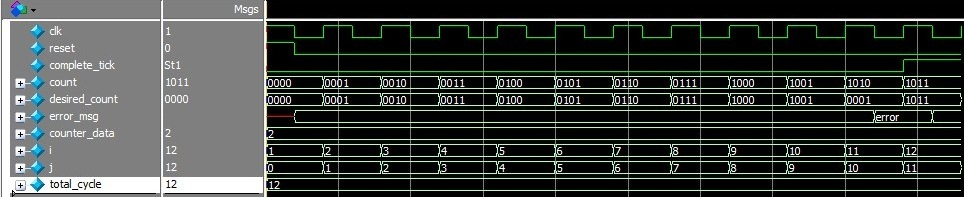
\includegraphics[width=\textwidth]{monitor_waveform}
		\caption{Waveform for Listing \ref{verilog:modMCounter_tb}}
		\label{fig:monitor_waveform}
	\end{figure}
	
	\begin{figure}[!h]
		\centering
		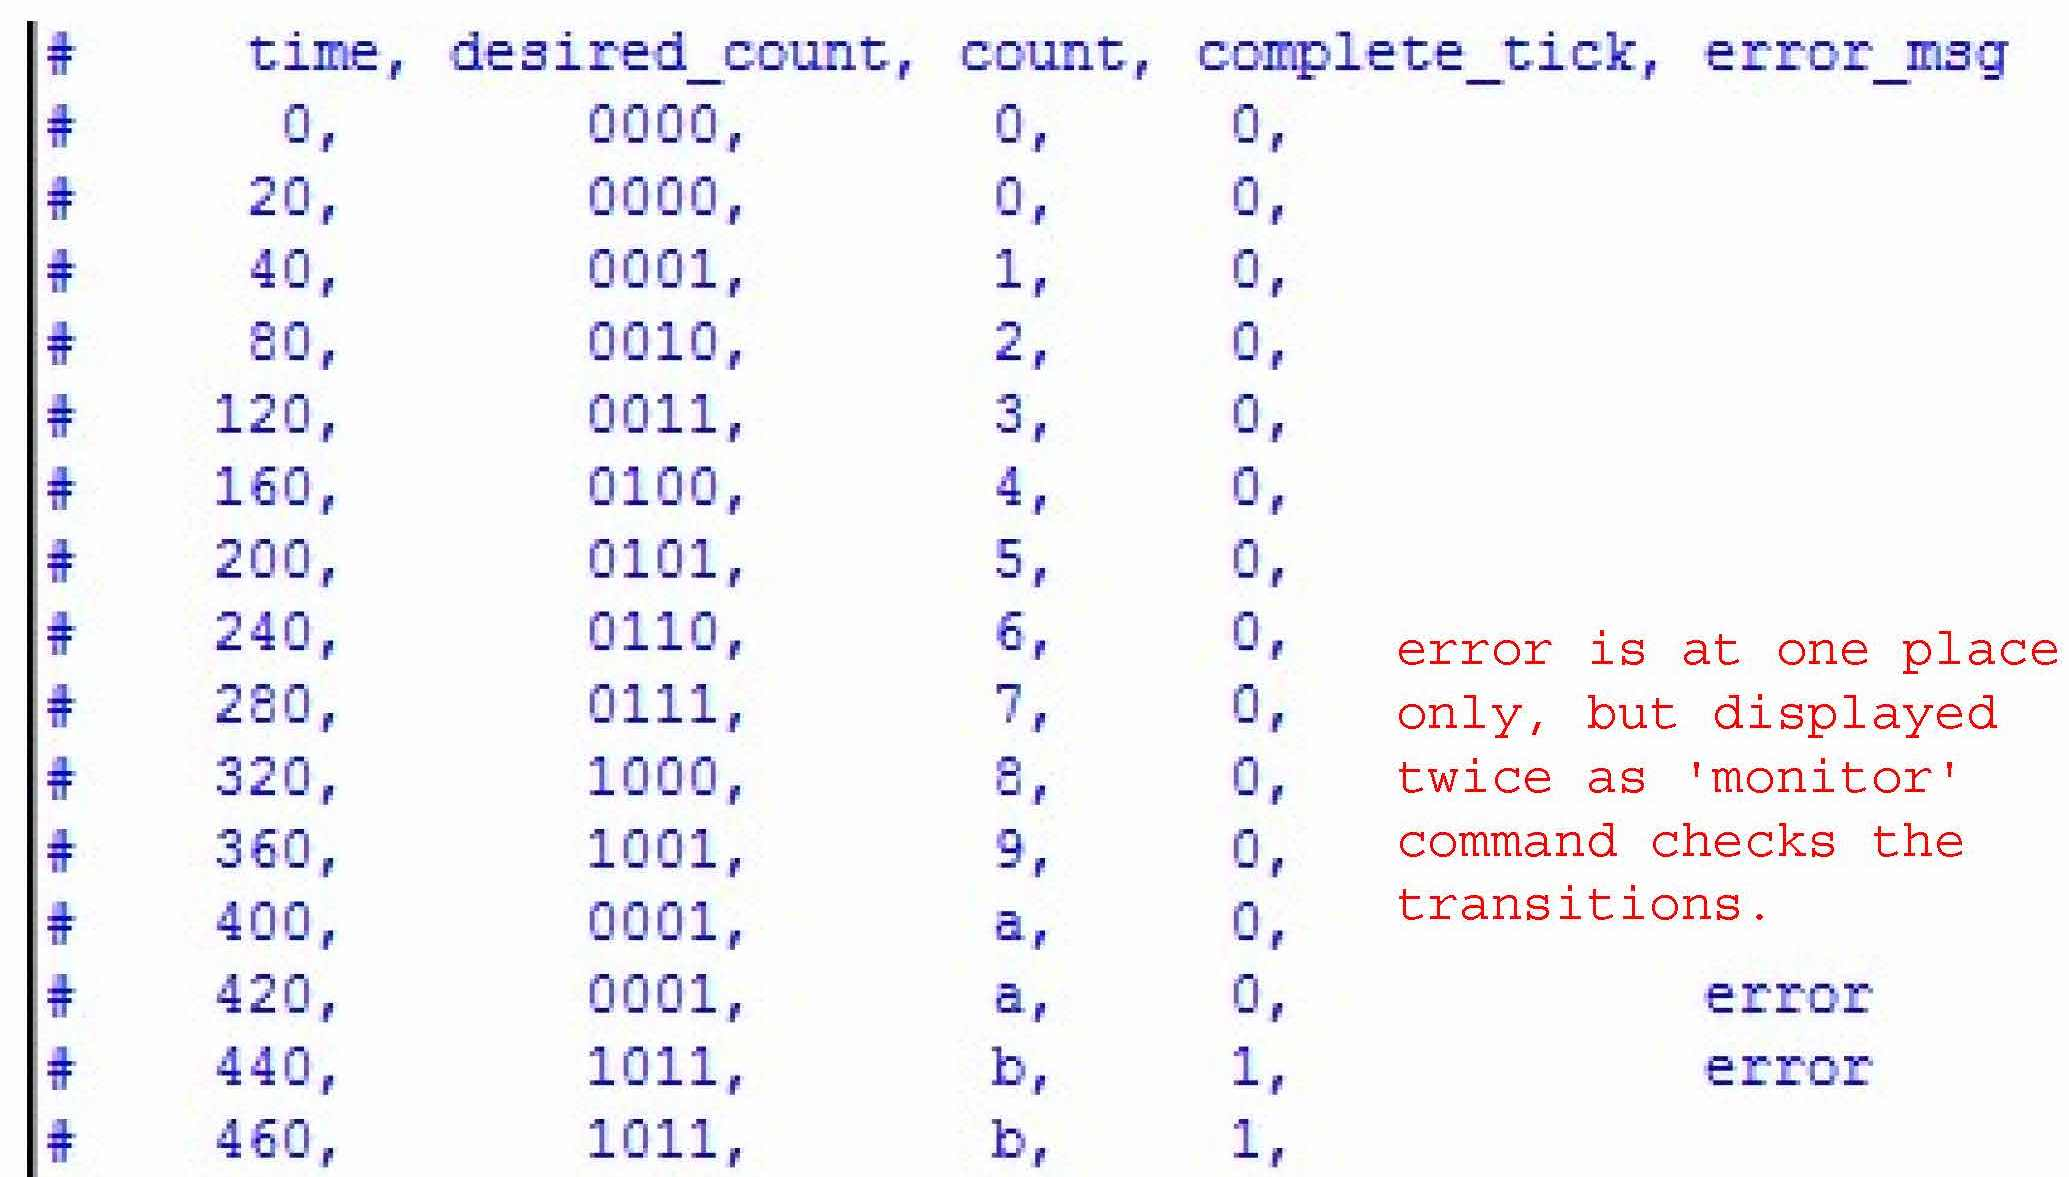
\includegraphics[scale=0.4]{monitor_error}
		\caption{Data displayed using `initial block' and `monitor' (Lines 98-108 of Listing \ref{verilog:modMCounter_tb})}
		\label{fig:monitor_error}
	\end{figure}
	
	\begin{figure}[!h]
		\centering
		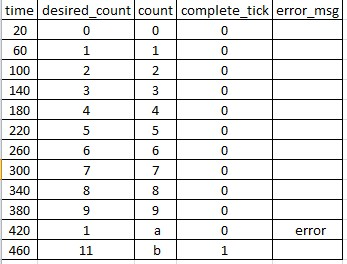
\includegraphics[scale=0.8]{error_neg_edge_csv}
		\caption{Data saved in .csv file using `always block' and `fdisplay' (Lines 110-124 of Listing \ref{verilog:modMCounter_tb})}
		\label{fig:error_neg_edge_csv}
	\end{figure}
	
	\begin{figure}[!h]
		\centering
		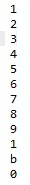
\includegraphics[scale=0.9]{content_mod_m_desire}
		\caption{Content of file `mod\_m\_counter\_desired.txt' }
		\label{fig:content_mod_m_desire}
	\end{figure}
	
\end{explanation}

\lstinputlisting[
language = Verilog,
caption    = {Save data of simulation},
label      = {verilog:modMCounter_tb}
]{modMCounter_tb.v}


\section{Conclusion}
In this chapter, we learn to write testbenches with different styles for combinational circuits and sequential circuits. We saw the methods by which inputs can be read from the file and the outputs can be written in the file. Simulation results and expected results are compared and saved in the csv file and displayed as simulation waveforms; which demonstrated that locating the errors in csv files is easier than the simulation waveforms.